\documentclass[../main.tex]{subfiles}

\begin{document}

\chapter[\hspace{0pt}绪\hskip\ccwd{}论]{{\heiti\zihao{3}\hspace{0pt}绪\hskip\ccwd{}论}}\label{chpt:intro}

本章内容共分为四节,\hyperref[section1: 研究背景及意义]{第一节}介绍本文的研究背景及意义;\hyperref[section1: 国内外研究现状与挑战]{第二节}总结少样本分类算法的国内外研究现状,并对其面临的挑战进行分析;\hyperref[section1: 本文研究内容与创新点]{第三节}介绍本文的研究内容与创新点;\hyperref[section1: 本文组织结构]{第四节}对本文组织结构进行概括。

\section[\hspace{-2pt}研究背景及意义]{{\heiti\zihao{-3} \hspace{-8pt}研究背景及意义}}\label{sec:reserach-background}

近年来,以深度学习为核心的人工智能技术取得了飞跃发展。其中,大规模预训练模型(如BERT、GPT系列)引领了自然语言处理等领域的范式变革,通过在海量数据上预训练模型再微调下游任务,大幅提升了各项任务性能。特别是大型语言模型(LLM)的兴起表明,模型规模和数据规模的扩张可以显著增强模型能力。以GPT-3为例,其参数规模高达1750亿,比前代GPT-2扩大两个数量级,并展示出少样本学习等新兴能力。研究指出,语言模型性能与模型参数规模、训练数据规模和计算量呈幂律关系持续提升。在过去几年中,SOTA模型的参数量正以每年至少10倍的速度增长,远超硬件性能提升速度。这一趋势导致模型训练成本飞速攀升——据估计,训练GPT-3单次迭代就需耗费约355 GPU年,费用超过\$460万美元。同时,模型参数存储和计算对显存和分布式计算提出了前所未有的挑战,模型并行化等新技术因此成为必要手段。

然而,追求规模效应的同时也暴露出效率瓶颈。首先,巨型模型的算力成本和能耗极为高昂,大模型开发仅有极少数科研机构和企业可承担。例如,中国北京智源研究院发布的“悟道2.0”多模态模型参数规模达1.75万亿,为GPT-3的10倍,采用了稀疏Mixture-of-Experts(MoE)架构以降低训练开销;即便如此,其训练仍消耗了海量的数据和算力资源。其次,模型对训练数据的依赖程度令人关注。大模型往往需要爬取、清洗数百GB乃至TB级的语料方能支撑预训练;而下游任务的有标签数据更为稀缺昂贵,许多场景难以获取足够的数据来微调如此庞大的模型。为缓解标注数据不足的问题,学术界提出了少样本学习、Prompt学习等方案,但这些方法通常仍依赖预训练模型的强大表征能力。

再次,即使有了预训练的大模型,将其迁移适配到特定任务或环境也面临困难。传统微调需要对模型全部参数进行梯度更新,但当模型参数量达到百亿级时,对每个新任务都进行全参数微调在计算和存储上都不可行。例如,针对一个1750亿参数的模型进行微调,不仅需要专用的多GPU集群支撑计算,其微调后的模型副本也难以部署。为提高适配效率,近年来出现了各种参数高效微调(PEFT)方法,例如冻结大部分预训练模型参数,仅在每层加入少量可训练参数的LoRA方法、在模型嵌入层追加可调向量的Prompt Tuning和Prefix Tuning等。LoRA将需要训练的参数数量减少了四个数量级,显著降低了显存占用和计算开销,在RoBERTa、GPT-3等上表现出与全模型微调相当的效果。同时,知识蒸馏等模型压缩技术作为一种经典的知识迁移手段,日益受到关注。蒸馏通过让小模型(学生)学习大模型(教师)的输出分布,实现模型压缩和加速,在移动设备等受限环境中具有重要意义。然而,小模型往往在模型容量和泛化性能上存在不足,蒸馏过程也需要精心设计(如教师选择、损失函数等)才能最大程度保留大模型知识。

此外,模型架构设计的复杂性也成为效率瓶颈之一。深度模型的性能高度依赖于网络架构,但手工设计高性能网络既需要专家经验又耗费大量试错成本。神经架构搜索(NAS)方法通过自动化搜索模型结构取得了一定成功,但经典NAS往往需要海量算力支撑,其搜索过程(如进化算法或强化学习控制器训练)可能耗费数千GPU天。为提高NAS效率,近年来提出了可迁移的NAS(Transferable NAS, TNAS),即利用先前搜索得到的知识来加速新任务上的架构搜索。然而现有TNAS大多局限于同构搜索空间(即假定新任务与旧任务在相同的网络搜索范围内)。当面对不同领域或不同搜索空间的新任务时,如何迁移架构设计经验仍缺乏有效手段,这导致跨领域NAS仍需从零开始,开销巨大。

最后,模型能力的迁移融合需求日益凸显。在实际应用中,一个预训练模型通常经过微调形成多个面向特定任务的专用模型,每个模型各司其职。然而这些微调模型之间缺乏协同,无法共享彼此学到的知识。传统上,如果希望一个模型同时解决多任务,往往需要进行多任务联合训练或增量训练,但这在大模型场景下成本同样高昂,且可能出现遗忘效应。为此,最近兴起了模型融合(Model Merging)技术,尝试在无需额外训练的情况下,通过直接融合多个已微调模型的参数来构造一个多任务统一模型。该思路在早期被称为“Task Arithmetic”(任务算术),即通过对模型参数向量进行算术运算来合成功能叠加的模型。然而,简单的参数平均或线性组合往往导致显著的性能退化,因为不同模型参数更新之间存在冲突和冗余。为解决这一问题,研究者提出了一系列改进策略。例如,Yadav等提出的TIES-Merging方法通过重置小幅更新参数、对齐符号冲突等步骤来减轻多模型融合时的干扰;Yu等提出的DARE方法则通过“Drop-And-Rescale”策略消除不同模型更新的不兼容部分,实现能力吸收。另外,Akiba等研究了利用进化算法自动优化融合配方,通过遗传搜索寻找最优的模型融合方式。尽管这些方法在一定程度上改善了多模型融合效果,但当融合的模型数量和任务范围继续扩大时,融合策略的搜索空间呈几何级膨胀,优化难度剧增,依然缺乏高效通用的解决方案。

综上所述,深度模型开发与适配面临“高成本、高复杂度”的严峻挑战:模型训练和微调的计算代价日益攀升,数据获取与标注成本巨大,模型架构设计与优化复杂耗时,多模型协同融合尚无成熟范式。这些背景和问题催生出强烈的研究动机——如何降低深度模型开发与适配的成本,让更广泛的任务和场景都能负担和受益于大模型的强大能力;如何高效地迁移已有知识和能力,避免重复训练并减小对海量数据的依赖;如何优化迁移过程以最大化迁移效果、避免负迁移和冲突。在这样的共同需求驱动下,本文将探讨新的理论和技术范式来应对上述挑战。

\section[\hspace{-2pt}核心科学问题]{{\heiti\zihao{-3} \hspace{-8pt}核心科学问题}}\label{sec:core-scientific-issues}

面对深度模型开发与应用中的种种效率瓶颈,本文关注的核心科学问题可以概括为:如何有效降低深度模型的开发与适配成本,通过知识迁移和优化手段来提升模型构建的效率和性能?具体而言,本研究试图解决以下关键问题:

\begin{enumerate}
  \item 如何高效地复用已有模型的知识来服务新的任务? 深度学习模型在源领域往往学得丰富的表征和能力,我们希望在目标任务中充分利用这些已有知识,而非从零开始训练。但不同任务/领域之间存在差异,直接迁移可能导致负迁移。需要研究迁移学习中“迁移什么、如何迁移、何时迁移”等基本问题,包括如何选择和提取源模型中对目标任务有用的知识(如特征、参数、结构)、如何设计高效的迁移策略和算法来避免源知识与目标任务冲突,以及在什么条件下迁移能带来正向增益。
  \item 如何降低大模型适配特定任务的资源开销? 传统的全模型微调在大模型场景下不可持续,需要探索参数高效的适配方法。例如只调优少量参数(如LoRA、Adapters)、借助少量示例的提示调优、或利用蒸馏将知识迁移到小模型以部署推理。核心问题在于如何在大幅减少训练开销的同时,最大限度保持原模型对新任务的性能。这里涉及到优化目标的权衡:既要减少计算量和参数改动,又要确保模型在目标任务上的准确率不显著下降。
  \item 如何实现在不同模型和架构之间迁移,以加速新模型的构建? 不同任务可能需要不同的模型结构,但从头设计和训练每个新架构代价巨大。如果能将之前任务中优化得到的架构设计经验迁移过来,将显著减少搜索时间。因此需要研究架构层面的迁移学习:包括如何表示和保存神经网络架构的知识,如何在新任务中高效利用这些知识初始化或引导架构搜索,如何跨不同搜索空间进行迁移等。这一问题延伸出对异构迁移(跨领域、跨架构)的探索,具有很强的挑战性。
  \item 如何将多个模型的能力融合到一个模型中? 当面对综合性任务或资源受限环境时,希望能有一个模型拥有多个已训练模型的技能,而不是维护多个专用模型。这涉及能力迁移与整合的问题:如何在不损失各模型特长的前提下,将它们融合为一个统一模型。需要解决参数冲突、能力干扰等技术难点,并寻找高效的融合优化方法来避免暴力搜索。这一问题连接到模型融合、终身学习、连续学习等研究方向,具有重要的理论和应用价值。
\end{enumerate}

概括而言,本论文要回答的核心问题是:能否提出一种统一的方法论,将模型知识迁移与优化过程有机结合,在内容、结构和系统层面全面提升深度模型开发与适配的效率? 这要求我们在理论上定义新的范式,在方法上提供可行的算法框架,并通过实验证明该范式在不同场景下的有效性。

\section[\hspace{-2pt}本文核心思想————迁移优化范式]{{\heiti\zihao{-3} \hspace{-8pt}本文核心思想}}\label{sec:core-idea}

针对上述科学问题,本文提出并定义一种统一的方法论——“迁移优化”(Transfer Optimization)范式。简而言之,迁移优化指的是:在深度模型的开发与适配过程中,以明确的优化目标为导向,将源模型/任务的知识高效迁移到目标模型/任务中,从而以最小代价获得最大性能增益的方法论。

这一范式包含“迁移”和“优化”两个关键词的有机结合。一方面,“迁移”强调利用已有的模型、数据或经验(记为迁移源 $S$)来帮助新的模型或任务(记为目标 $T$),体现为知识层面的重用;另一方面,“优化”则意味着我们并非简单地直接套用源知识,而是围绕某个性能指标或损失函数(记为优化目标 $F(\cdot)$)来主动调整迁移过程,通过算法优化使迁移效果最优。

具体来说,我们将迁移优化范式应用于深度模型开发与适配的不同层面,呈现出方法论的统一性:

\begin{itemize}
  \item \textbf{模型知识迁移(内容优化):}这是迁移优化在\textit{知识内容}层面的体现。典型情形如知识蒸馏,我们以大模型的预测分布或中间表示为知识 $K$,通过设计特定的损失函数 $F$ 来优化学生模型对这些知识的拟合,从而在保持性能的情况下压缩模型。又如微调优化,我们冻结部分参数,仅优化少量新参数,使模型在新任务上的损失 $F$ 最小化。这些过程都符合迁移优化的范式:从源模型提取有价值的知识,并通过优化算法高效传递给目标模型。本文的工作1(详见第3章)正是关注于此,通过对比学习优化目标,实现在少样本条件下大模型对小模型的知识迁移。
  \item \textbf{模型架构迁移(结构优化):}这是迁移优化在\textit{模型结构}层面的应用。传统NAS需要从头搜索架构,而迁移优化范式下,我们希望将源任务中优良架构的设计经验迁移过来。例如,可将已验证有效的网络模块、拓扑等作为先验嵌入到新任务的搜索过程中,并设定适当的优化目标 $F$ 引导搜索,使得在更小搜索成本下找到高性能架构。这种方法论上的统一在可迁移架构搜索中得到体现。本文的工作2(详见第4章)提出了跨搜索空间的迁移NAS方法,通过学习公共的架构表示和演化优化算法,实现不同任务之间架构知识的迁移,被视为迁移优化在结构设计上的成功实践。
  \item \textbf{模型能力迁移(系统级优化):}这是迁移优化在\textit{系统整合}层面的体现。它关注将多个模型的能力迁移并融合到一个模型中,涉及复杂的多源迁移情景。迁移优化范式认为,可以通过将多模型融合问题转化为一个优化问题,设定合理的目标函数(例如融合后模型在各任务上的综合损失),并利用优化算法在参数空间中搜索最优的融合方案。这一思想贯穿于模型融合最新研究中,例如上文提到的TIES-Merging通过优化参数符号一致性来减小干扰,Akiba等的进化融合通过遗传算法优化融合配比。在本文工作3(详见第5章)中,我们同样遵循迁移优化范式,将大模型多任务融合表述为多个子问题的优化组合,借助演化策略逐步迁移各子问题的解以优化原问题,实现了系统级能力的高效整合。
\end{itemize}

通过以上三方面,我们正式定义迁移优化为一个普适的方法论范式:给定迁移源 $S$(可以是预训练模型、已有架构、已训好的模型集合等)和目标 $T$(可以是新模型、新任务域或融合后的模型),确定待迁移的知识元素 $K$(如参数、特征、结构单元等)以及任务域 $D$(如数据分布、任务集合),设计适当的优化目标函数 $F(\cdot)$,并通过优化算法求解,使得知识从 $S$ 向 $T$ 的传递效果达到最优。在这个范式下,不同迁移场景中的众多方法都可视作特例:无论是知识蒸馏、参数高效微调,还是架构搜索迁移、模型融合等,都可以抽象为上述形式。这种统一性有助于我们从更高的视角审视深度学习中的迁移问题,并开发出兼具通用性和高效性的解决方案。值得注意的是,在进化计算领域也出现了将知识迁移融入优化过程的研究,被称为“进化迁移优化”。本文的迁移优化范式在思想上与其一脉相承,但我们聚焦于深度模型领域的迁移与优化融合,涵盖模型训练、架构设计和模型融合等多个层面,具有更广泛的应用背景和挑战。

\section[\hspace{-2pt}本文研究内容与主要贡献]{{\heiti\zihao{-3} \hspace{-8pt}本文研究内容与主要贡献}}\label{sec:research-content-and-contribution}

\section[\hspace{-2pt}本文结构安排与符号约定]{{\heiti\zihao{-3} \hspace{-8pt}本文结构安排与符号约定}}\label{sec:structure-and-symbols}



\end{document}

% \section[\hspace{-2pt}研究背景及意义]{{\heiti\zihao{-3} \hspace{-8pt}研究背景及意义}}\label{section1: 研究背景及意义}

% \section[\hspace{-2pt}国内外研究现状与挑战]{{\heiti\zihao{-3} \hspace{-8pt}国内外研究现状与挑战}}\label{section1: 国内外研究现状与挑战}

% \subsection[\hspace{-2pt}研究现状]{{\heiti\zihao{4} \hspace{-8pt}研究现状}}\label{section1: 研究现状}

% 近年来,已有很多少样本分类方法被提出,按其技术方案可以大致分为五类,分别是:基于元学习的少样本算法、基于度量的少样本算法、基于数据增强的少样本算法、基于特征学习的少样本算法和基于语义的少样本算法,以下将分别对其进行介绍。

% \textbf{(1)基于元学习的少样本算法}

% 基于元学习的少样本分类算法\cite{MAML, lee2019meta, LEO, 元学习},其核心思想是在训练阶段便模拟少样本测试任务,在从基类数据集采样的大量少样本分类任务中学习到元知识,元知识可以迁移到其他少样本任务,从而使模型在遇到新任务时能够通过极少量的样本训练便快速调整参数并达到较好的分类性能。例如,Finn等人\cite{MAML}提出了模型无关的元学习算法(Model-Agnostic Meta-Learning,简称 MAML)。MAML设计了一种优化算法,通过找到一组初始化模型参数,使用少量梯度下降便能够使其适应新的任务。Lee等人\cite{lee2019meta}则是使用支持向量机(Support Vector Machine,简称SVM)代替MAML方法中的线性分类器,并结合了一个可微分二次规划求解器使得其能够端到端学习。Rusu等人\cite{LEO}提出了一种在低维潜在空间进行模型元学习的方法LEO,其将元学习问题转化为潜在空间中的优化问题,利用潜在空间的特征嵌入捕捉少样本任务间共享的结构性知识,促进不同任务间的知识转移。基于元学习的方法虽很符合少样本分类的特点,但其通常需要先对特征提取网络进行预训练,并在元学习阶段采样大量任务来微调网络,存在训练过程较为复杂的问题。

% \textbf{(2)基于度量的少样本算法}

% 基于度量的方法\cite{ProtoNet, vinyals2016matching, DeepEMD, 度量学习}为少样本分类问题提供了另一种解决思路,其旨在通过学习样本之间的距离或相似度度量来处理少样本问题。这类方法的核心思想是,如果能够合理地度量样本之间的距离或相似性,即便是只有少量的训练样本,也可以通过比较未知样本与已知样本之间的距离或相似度来进行有效的分类。基于度量的方法大多使用欧式距离、余弦相似度计算样本之间的距离,例如Snell等人\cite{ProtoNet}提出的原型网络(Prototypical Networks, 简称ProtoNet)。ProtoNet基于以下假设:在特征空间中,每个类别都可以由其样本特征的平均值代表的一个原型来表示。在进行分类时,其会计算查询样本与每个类别原型之间的欧式距离,并将查询样本分类到最近的原型所代表的类别。Zhang等人\cite{DeepEMD}提出的DeepEMD方法为少样本分类引入了一种新的距离度量方式:推土机距离(Earth Mover's Distance,简称EMD)。DeepEMD将一张图像分为不同的图像块,对其进行特征提取并利用推土机距离作为度量标准来比较不同图像之间的相似度。另外,Sung等人\cite{RelationNet}提出的关系网络(Relation Networks,简称RelationNet)则是通过学习一个深度度量来评估样本之间的关系得分,进而通过关系得分进行分类。与之前方法不同,此关系得分是通过网络学习到的,而不是设计的固定距离度量方式。基于度量的少样本算法简单高效,其难点主要在于如何建立一个合适的度量方式来衡量样本之间的距离或相似度。

% \textbf{(3)基于数据增强的少样本算法}

% 增加样本数量来应对标注样本不足的问题,是少样本分类最直观的解决方案,因此,基于数据增强的少样本算法被提出\cite{IDeMe-Net, AFHN}。少样本分类中,每个类别样本数目极少,模型很容易产生过拟合问题,该类算法通过增加训练样本的数量和多样性来帮助模型学习到更加鲁棒的特征表示,从而减少过拟合的风险。例如,Chen等人\cite{IDeMe-Net}提出了一种名为图像变形元网络(Image Deformation Meta-Networks,简称IDeMe-Net)的新颖框架。IDeMe-Net训练一个网络,该网络能够通过线性地融合一组图像生成变形图像,从而产生额外的标注样本,增加模型的训练样本。Li等人\cite{AFHN}提出的对抗性特征幻觉网络(Adversarial Feature Hallucination Networks,简称AFHN)则是在特征层次对样本数量进行增加。AFHN方法利用生成对抗网络(Generative Adversarial Nets,简称GAN)\cite{GAN}来生成新的样本特征,从而解决训练样本特征稀缺的问题。另外,还有部分方法将语义信息作为条件并使用生成模型合成额外的训练样本或特征,由于此类方法使用到了语义信息,因此将其划分为基于语义的少样本算法,将在后续进行介绍。基于数据增强的方法更符合解决少样本分类问题的直觉,但其需要增加很多样本以缓解过拟合问题,并且如何确保所增加样本的多样性也是一大挑战。

% \textbf{(4)基于特征学习的少样本算法}

% 近年来,少样本分类的特征学习阶段越来越受到重视,并出现了一系列基于特征学习的少样本算法\cite{RFS,chencloser, dhillon2019baseline, HandCrafted, IER, PAL, Spatial, FSLwCL, SSLforFSL, DeepBDC}。这些方法直接使用整个基础数据集以和普通分类任务一致的方式来训练模型,直接执行分类任务或者增加额外的辅助任务以获得特征提取能力出色的特征提取网络。Tian等人\cite{RFS}总结了基于元学习以及度量学习方法的不足,并开创性地提出RFS方法。RFS在整个基类数据集上执行分类任务训练网络来学习良好的特征嵌入,在测试阶段,RFS冻结特征提取网络参数并使用其提取图像特征,并随后添加逻辑回归分类器进行少样本分类任务。通过此种简单的方式便可得到一个优质的特征提取网络,并能够达到良好的少样本分类结果。在此基础上,一些其他人的工作\cite{chencloser, dhillon2019baseline}进一步证明了此类方法的有效性。另外,还有一些工作在分类任务的基础上添加额外的辅助任务进一步提升特征提取网络的泛化性。例如,Zhang等人\cite{HandCrafted}提出使用方向梯度直方图(Histogram of Oriented Gradient,简称HOG)和局部二值模式(Local Binary Patter,简称LBP)来提取手工特征并用来指导特征提取网络的优化,缓解了模型的过拟合问题。其他一些工作\cite{IER, PAL, Spatial, FSLwCL, SSLforFSL, DeepBDC}则是利用自监督或者对比学习任务作为辅助任务来提升模型的特征提取能力以及泛化能力,从而达到良好的少样本分类表现。相比于基于元学习、度量和数据增强的方法,基于特征学习的方法对少样本分类提供了一种更为简单的解决方案,但目前部分方法仅使用分类损失训练网络或者直接使用一些对比学习的方法辅助训练,没有对样本关系进行充分挖掘,限制了模型性能。

% \textbf{(5)基于语义的少样本算法}

% 受到人类认知新类别时语义信息可以提供帮助作用的启发,研究者开始将语义信息引入到少样本分类算法中。基于语义的少样本算法通常使用Word2Vec\cite{Word2Vec}、GloVe\cite{GloVe}、BERT\cite{Bert}等自然语言模型或者CLIP\cite{Clip}等多模态模型的文本编码器来将类别名称转化为语义特征,并使用其对视觉特征进行补充以使得模型能够获取样本的多种模态信息,丰富了样本特征所包含的信息,进而可以提高少样本分类准确率。根据其利用语义信息的方式不同,本文将其大致分为两类,分别是基于特征生成的方法和基于语义修正的方法。

% \textbf{基于特征生成的方法:} 此类方法将语义信息作为生成模型的条件生成额外的样本以提升样本多样性,从而缓解分类器仅用少量样本训练容易出现过拟合的问题。例如,Chen等人\cite{DualTriNet}将编码器提取的多层视觉特征映射到语义空间,在语义空间使用语义信息对映射后的视觉特征进行特征增强后再用一个解码器将其映射回视觉空间并得到增强后的特征,使用增强后的特征与原始特征共同训练分类器从而达到特征增强的目的。Zhang等人\cite{STVAE}提出的STVAE模型则是使用不同维度的先验知识(包括视觉先验和语义先验)分别作为变分自编码器(Variational Auto Encoder,简称VAE)的生成条件生成特征并对其进行融合得到最终的生成特征,将生成的特征作为额外的训练样本以增加样本多样性。

% \textbf{基于语义修正的方法:} 此类方法的核心思想在于通过约束或者融合的方式利用语义信息对视觉特征进行修正,以优化模型对样本的理解和分类能力,提升模型的泛化能力。例如,Xing等人\cite{AM3}设计了一种自适应融合机制,该机制能够根据需要学习的新图像的类别自适应地融合视觉信息与语义信息,从而捕获视觉、语义两种模态空间的互补信息,增强模型在新类别上的识别能力。另外,Chen等人\cite{SP-CLIP}则是将语义信息作为额外输入,与样本图像一同输入模型,并设计了空间维度以及通道维度两种互补机制,以利用语义特征作为提示自适应地调整视觉特征提取网络以及对视觉特征进行补充,从而获得更全面的样本特征,提升模型的少样本分类准确率。

% 总的来说,基于语义的少样本算法引入了语义信息,能够对视觉信息进行补充,丰富了模型获取信息的来源,但如何更简单有效地利用语义信息需要进一步探讨。

% \subsection[\hspace{-2pt}研究挑战]{{\heiti\zihao{4} \hspace{-8pt}研究挑战}}\label{section1: 研究挑战}

% 通过对国内外研究现状进行分析,本文认为当前少样本分类问题还存在着以下挑战:

% (1)少样本分类中,训练一个强大的特征提取网络十分重要,它决定了特征的判别性以及模型的泛化性。然而,目前部分少样本方法对于特征学习阶段关注不够,或直接使用一些通用的特征学习方法训练模型,使得在基类上训练的模型在新类上的特征提取能力不足。因此,如何使用基类数据训练一个迁移能力强、泛化性能好的特征提取网络是当前少样本分类面临的一个挑战。

% (2)由于在新类执行少样本分类任务时,采样的任务标注样本数量极少,仅仅根据少量样本的视觉特征可能无法捕获类别的代表性特征,因此很多方法引入语义信息以对视觉信息进行补充,进而提高模型在新类上的泛化能力。但如何设计一种简单有效的手段既能够利用语义信息丰富样本特征的信息来源,又不需要复杂的训练流程及模块设计仍需要进一步探讨。

% \section[\hspace{-2pt}本文研究内容与创新点]{{\heiti\zihao{-3} \hspace{-8pt}本文研究内容与创新点}}\label{section1: 本文研究内容与创新点}

% 鉴于当前少样本分类问题中存在的模型特征提取能力不够强、少量样本视觉特征不具有代表性的问题,本文致力于通过充分挖掘数据间的多元关系对其进行解决。本文通过研究基于多元关系建模的少样本分类算法,以对基类与新类共享的深层次数据关系进行挖掘,从而理解数据间的内在联系,将在基类数据上学习到的知识更好地迁移至新类,提升模型在数据匮乏的新类上的分类性能。基于此,本文分别对多粒度样本关系以及语义-视觉多空间关系进行了建模,充分有效地利用了样本间的不同关系以及语义信息,提升了模型的特征提取能力和泛化能力。本文研究内容详细介绍如下:

% \textbf{(1)基于多粒度样本关系建模的少样本分类研究}

% 针对少样本分类模型特征提取能力不足的问题,本文提出了一种多粒度样本关系对比学习(Multi-Grained Sample Relation Contrastive Learning,简称MGSRCL)方法,旨在对不同粒度的样本关系进行建模以提升模型的知识迁移能力。MGSRCL方法将样本关系细致地划分为三种:同一样本不同变换版本之间的样本内关系、同类样本的类内关系和不同类样本的类间关系。通过对不同样本关系针对性地设计对比学习任务,MGSRCL合理地对多种粒度的样本关系进行约束和优化,提升了模型所提取特征的判别性和泛化性。在miniImageNet\cite{vinyals2016matching}、tierdImageNet\cite{ren2018meta}、CIFAR-FS\cite{bertinetto2019meta}和CUB-200-2011\cite{wah2011caltech}四个少样本分类基准数据集上的大量实验表明,MGSRCL方法通过充分挖掘样本关系提升了模型的特征提取能力,达到了优异的分类准确率。

% \textbf{(2)基于语义-视觉多空间关系建模的少样本分类研究}

% 针对仅根据少量样本的视觉特征无法捕获类别代表性特征的问题,本文进一步引入语义信息作为视觉信息的补充,提出了语义-视觉多空间映射适配(Semantic-Visual Multi-Space Mapping Adapter,简称SVMSMA)模型。该模型利用自然语言模型或多模态模型的文本编码器提取语义信息,将其通过语义-视觉多空间映射网络映射到视觉空间,并设计跨模态分类和特征对齐策略,使模型能够对语义信息与视觉信息的关系进行建模,丰富了样本特征的信息来源,使其更具有代表性,从而增强了模型对新类别的适应性和泛化能力。本方法同样在四个少样本分类基准数据集进行了大量实验,在MGSRCL模型的基础上取得了进一步的性能提升。

% 本文提出的MGSRCL模型与SVMSMA模型分别从多粒度样本关系和语义-视觉多空间关系两个角度出发,对少样本分类中的多元关系进行了深入挖掘与研究。MGSRCL模型通过对多种粒度的样本关系进行不同的对比学习任务,对数据间的多种样本关系进行有效建模,提升了模型的特征提取能力;SVMSMA模型则进一步引入类别的语义信息,使用两种跨模态任务对数据在语义与视觉不同空间之间的关系进行建模,提高了模型的泛化能力。通过这两个模型,本文有效地利用了数据中的多元关系,取得了较好的少样本分类结果。

% 本文的创新之处主要体现在以下两个方面:

% (1)多粒度样本关系的深入挖掘:重新对样本关系进行了思考与划分并提出了基于样本内关系、类内关系和类间关系的多粒度样本关系对比学习方法,充分利用了样本之间复杂且多样的关系,为少样本分类提供了一个有效的特征学习方法。

% (2)语义-视觉多空间关系的建模:通过融合语义信息和视觉信息,提出了一种简单有效的少样本分类模型,该模型可以通过跨模态的特征学习和原型对齐,有效利用语义信息对视觉信息进行补充,从而进一步提升少样本分类的性能。

% \begin{figure}[h]
%   \centering
%   \captionsetup{font={small, stretch=1.312}}
%   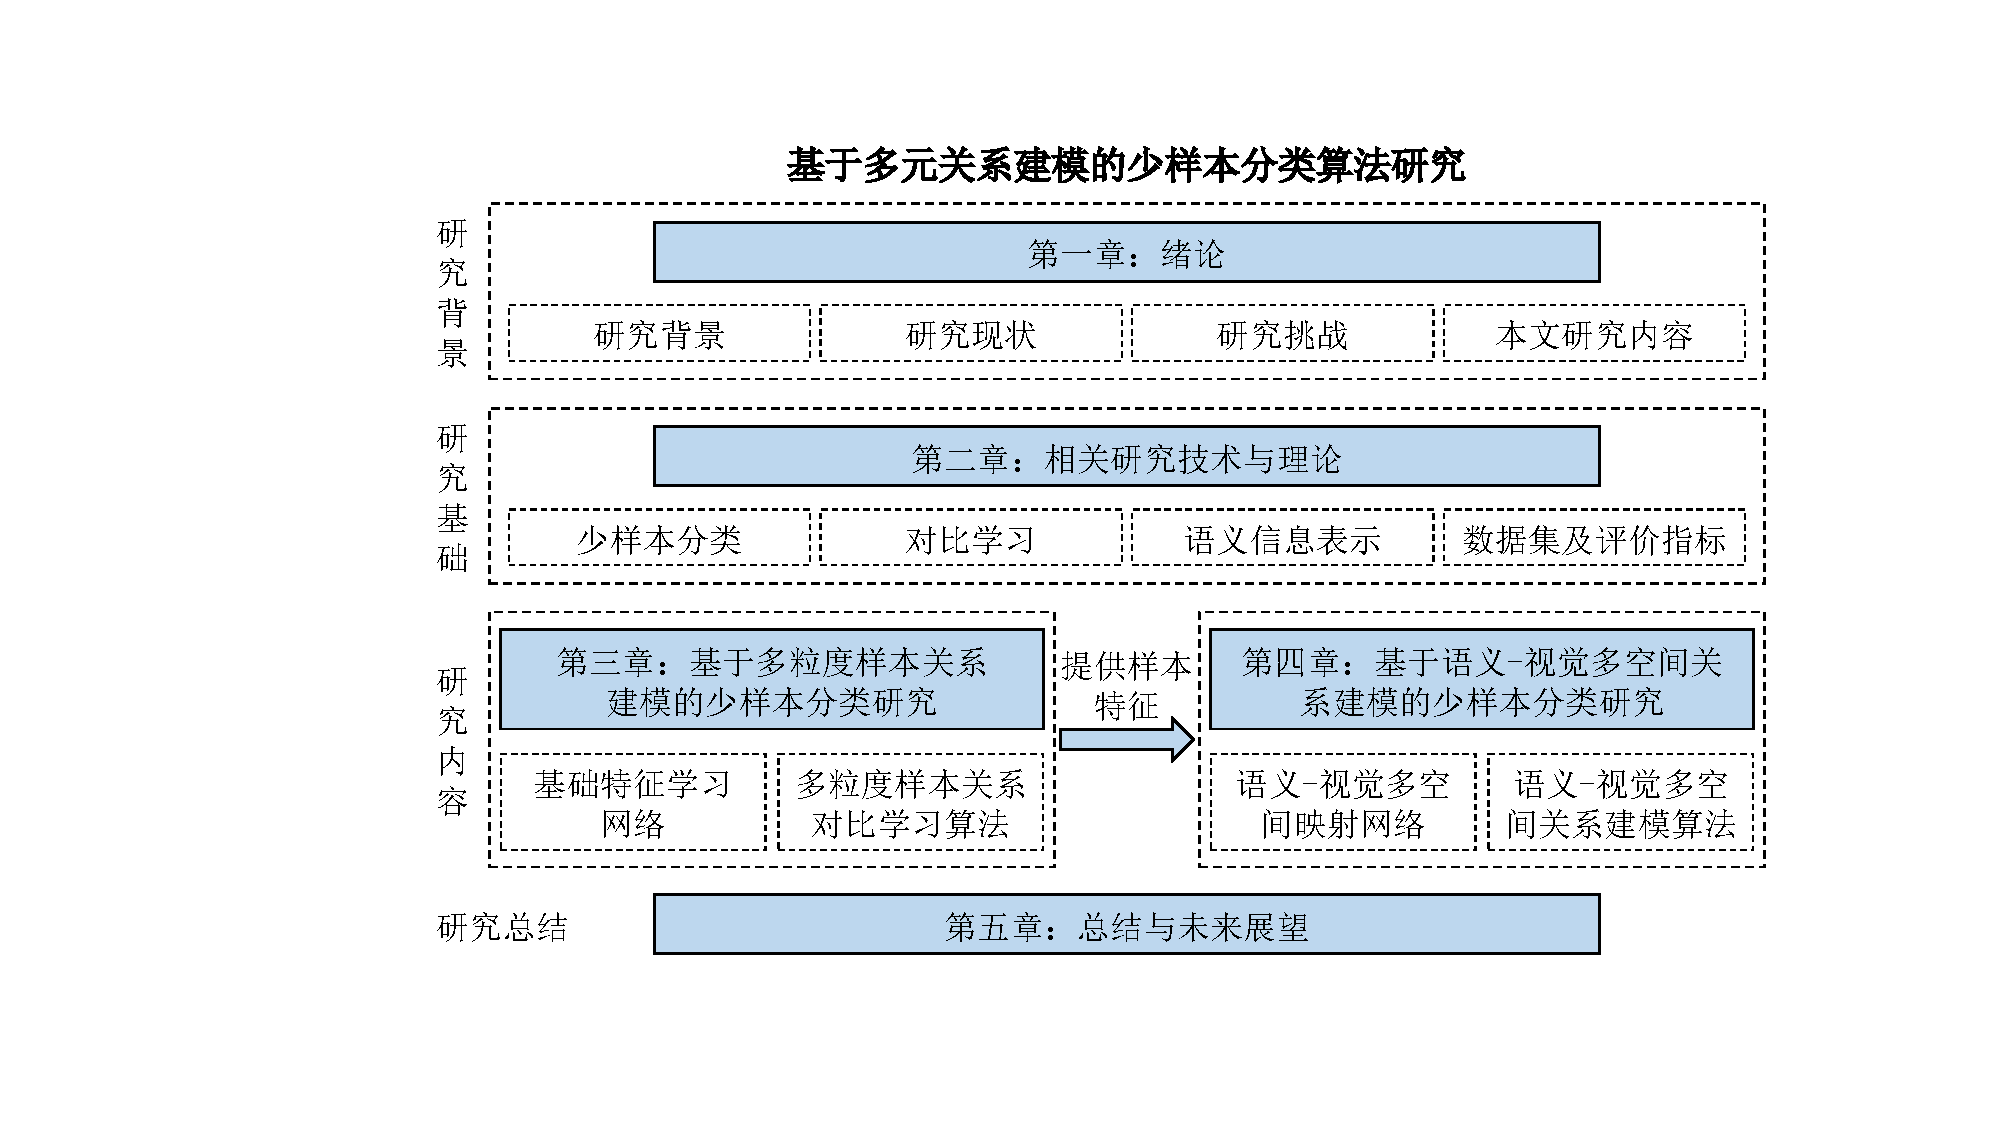
\includegraphics[width=1.0\columnwidth]{figures/组织结构.pdf}
%   \bicaption[本文组织结构图]{本文组织结构图。}[The organizational structure of the paper]{The organizational structure of the paper.}
%   \label{figure1: 组织结构}
% \end{figure}

% \section[\hspace{-2pt}本文组织结构]{{\heiti\zihao{-3} \hspace{-8pt}本文的组织结构}}\label{section1: 本文组织结构}

% 本文的组织结构图如图\ref{figure1: 组织结构}所示,共分为5个章节,各章节的介绍如下:

% 第一章:绪论。介绍少样本分类的研究背景和意义,并分析总结少样本分类算法的国内外研究现状及存在的挑战。最后对本文的研究内容和组织结构进行概述。

% 第二章:相关研究技术与理论。首先对少样本分类进行了进一步详细介绍,然后介绍本文方法中所使用到的对比学习技术以及语义信息表示,最后对本文实验所使用到的数据集及评价指标进行介绍。

% 第三章:基于多粒度样本关系建模的少样本分类研究。首先对部分现有少样本特征学习算法的不足进行分析,提出了基于多粒度样本关系对比学习的少样本特征学习算法(MGSRCL),随后详细介绍了针对不同粒度样本关系的建模方法,最后通过在四个基准数据集的大量实验证明了MGSRCL模型的有效性。

% 第四章:基于语义-视觉多空间关系建模的少样本分类研究。首先对基于语义的少样本分类算法进行分析介绍,提出了基于语义-视觉多空间关系建模的少样本特征适配算法(SVMSMA),然后介绍了SVMSMA模型的模型框架以及提出的跨模态分类和跨模态特征对齐模块,最后对所提方法进行了实验分析。

% 第五章:总结与未来展望。总结并分析了本文提出的基于多元关系建模的少样本分类算法研究的成果及不足,并对未来的研究方向与内容进行了展望。
